\documentclass[fleqn]{article}
\pagenumbering{arabic}

%\usepackage{showkeys}
\usepackage{url}
\usepackage{graphicx}
\usepackage{fullpage}
\usepackage{html}
\usepackage[T1]{fontenc}
\usepackage [latin2]{inputenc}
\usepackage {times}
\usepackage{dsfont}
%\usepackage[english]{babel}
\usepackage {amsmath}
\usepackage {amsthm}
\usepackage {amssymb}

\def \R {\mathbb R}
\def \NnP {\mathbb P}
\def \N {\mathbb N}
\def \Real {\textrm{Re}}
\def \C {\mathbb C}
\def \tr {\textrm{tr}}
\def \aff {\textrm{aff}}
\def \ri {\textrm{ri}}
\def \co {\textrm{co}}
\def \diag {\textrm{diag}}
\def \sgn {\textrm{sgn}}
\def \E {\mathbb{E}}
\def \I {\mathds{1}}

\newtheorem{tetel}{T�tel}
\newtheorem{lemma}[tetel]{Lemma} %Ennek hat�s�ra a T�tel �s Lemma sorsz�mok egym�st k�vetik
\newtheorem{segtetel}[tetel]{Seg�dt�tel}
\newtheorem{defi}{Defin�ci�}
\newtheorem*{megj}{Megjegyz�s} %A csillag hat�s�ra nem kap sorsz�mot
\newtheorem*{kov}{K�vetkezm�ny}
\newtheorem*{pelda}{P�lda}
\newtheorem{all}[tetel]{�ll�t�s}
\newtheorem{algo}{Algoritmus}

\newtheorem{prop}{Proposition}
\newtheorem{stat}{Statement}
\newtheorem{defin}{Definition}
\newtheorem{thm}{Theorem}
\newtheorem{ass}{Assumption}


\renewcommand{\baselinestretch}{1.2}

\newcommand{\figref}[1]{\ref{#1}. \figurename~}
\newcommand{\argmin}{\operatornamewithlimits{argmin}}
\newcommand{\secref}[1]{Section \ref{#1}}


\newenvironment{source}
{\begin{list}{}{\setlength{\leftmargin}{1em}}\item\scriptsize\bfseries}
{\end{list}}

\newenvironment{tinysource}
{\begin{list}{}{\setlength{\leftmargin}{1em}}\item\tiny\bfseries}
{\end{list}}

\usepackage {bm}
%\usepackage{paralist}
\title{SPSToolbox - User Manual}
\author{S�ndor Kolumb�n}

%\begin{figure}[htb]
% \centerline{\includegraphics[width=.7\columnwidth]{Figures/normx50.jpg}}
% \caption{The difference of the internal estimates of $x$ from the final value}
% \label{fig:xnorm}
%\end{figure}


\begin{document}

\pagestyle{plain}
\maketitle

\tableofcontents


\section*{Versions}

\begin{tabular}{|l|l|l|}
  \hline
  % after \\: \hline or \cline{col1-col2} \cline{col3-col4} ...
  Date & Author & Contribution \\
  \hline
  30. 04. 2013 & Kolumb�n & Initial version\\
  \hline
\end{tabular}

\section{Introduction}

This document briefly introduces a hypothesis testing procedure called sign perturbed sums (SPS) and describes the use of the Matlab Toolbox that implements it. The method was developed in a series of papers \cite{Csaji2012Sysid, Csaji2012CDC, Kolumban2013CDC}. The method allows hypothesis testing of parameters in case of linear regression problems and in case of LTI Box Jenkins models (\cite{ljung1999SysId}). The important features of the method are that the only assumption about the noise or error values is that they have symmetric distribution about zero and that no asymptotic theory is used. This means that the confidence of the hypothesis test is rigorous.

For instruction on installation see Section~\ref{sec:Deploy}.

The structure of the manual is as follows. Section~\ref{sec:ShortDescr} illustrates the principles of the algorithm without going into details on a toy example. More details can be found in the cited references. The methods provided by the toolbox and their usage is presented in Section~\ref{sec:Usage} and examples are given in Section~\ref{sec:Ex}.

\section{Short description of the theory}
\label{sec:ShortDescr}

In order to introduce the terminology, this section briefly presents the SPS method on a toy example. We show the steps of the method here and illustrate them on the simple one parameter problem
\[
y_k = \theta_0 + n_k \qquad k=1, \ldots, N
\]
Some of these steps are redundant in case of this toy example but in case of linear dynamical systems parameter estimation they are needed. We want to create a confidence test for a model parameter $\theta$ on confidence level $1-q/m$. The steps of the algorithm are the following.

1. $m-1$ random sign sequences of length $N$ and a random permutation of length $m$ should be generated.
\[
\alpha(i,k) = 2 \ \textrm{round(RAND)}-1 \qquad i=1,\ldots, m-1 \quad k=1, \ldots, N
\]
$\alpha(0, k) = 1$ is the first sign sequence and it is fixed.

2. Compute the noise sequence $\hat{N}_k(\theta) $ corresponding to the data and the tested model.
\[
\hat{N}_k(\theta) = y_k - \theta
\]

3. Create perturbed noise sequences based on $\hat{N}_k(\theta)$
\[
\hat{N}^{(i)}_k(\theta) = \alpha(i,k)\hat{N}_k(\theta) = \alpha(i,k)(y_k - \theta)
\]

4. Using the perturbed noise sequences, create perturbed versions of the measurements
\[
\hat{Y}^{(i)}_k(\theta) = \theta + \hat{N}_k(\theta) = \theta +  \alpha(i,k)(y_k - \theta)
\]

Quadratic cost function is used for the estimation of the unknown parameter. The estimation is given by the solution of the normal equation to this. For each noise realization there is a different cost function and a different normal equation. It is important that from this point on there are $m$ independent identification problems that are considered.
\[
J^{(i)} = \sum_{k=1}^N (\hat{Y}^{(i)}_k(\theta) - \theta)^2
\]

5. Calculate the gradient of the prediction errors. In this simple example these are
\[
\psi_k^{(i)} = -1
\]

6. Compute the perturbed covariance estimate
\[
\Psi^{(i)} = \frac{1}{N} \sum_{k=1}^N \psi_k^{(i)}  \left[\psi_k^{(i)} \right]^T = 1
\]

7. Calculate the normal equation of the cost function
\[
\frac{\partial J^{(i)}}{\partial \theta} =  \sum_{k=1}^N -2\left(\hat{Y}^{(i)}_k(\theta) - \theta \right) = 0
\]

8. The $S_i$ values are the gradient vectors of the cost function at $\theta$ in the different identification scenarios.
\[
S_i = \sum_{k=1}^N -2 \hat{Y}^{(i)}_k(\theta) + 2 N \theta =
      \sum_{k=1}^N -2 \left[ \theta + \alpha(i,k)(y_k - \theta)\right] + 2 N \theta =
      \sum_{k=1}^N -2 \alpha(i,k)(y_k - \theta)
\]

9. Create the different $Z_i$ values which measure the length of the gradient weighted with the inverse of the covariance matrix
\[
Z_i = S_i^T \left[\Psi^{(i)}\right]^{-1} S_i = S_i^2
\]

10. Order the different $Z_i$ values in descending order. In case of ties use the random permutation generated at the beginning the make the ordering explicit.

11. If $Z_0$ is between the $m$ largest $Z$ value, then the model $\theta$ is no part of the confidence set.

Since the LS estimate of the original problem will make $Z_0=0$, it will always be inside the set. 

The basic underlying idea is that $m$ different identification problems are created. From the perspective of $\theta_0$ these are identically distributed as the original problem and they are also independent from each other (showing this is a bit more technical). We calculate the gradient of the objective function of the considered model $\theta$ on each identification problem ($S_i$) and measure their length $Z_i$. We say that the selected model is pretty good if it is closer to solving the original problem than the other ones.

As we go to infinity with $\theta$ it is easy to see in this simple case that $Z_0$ will outgrow every other $Z$ value as the coefficient of $\theta$ is the largest here in absolute value.

\pagebreak

\section{Using the toolbox}
\label{sec:Usage}

This section describes the functionality of methods belonging to the toolbox. The main functions of the toolbox are
\begin{itemize}
\item GenerateSPSSetup: generates the random quantities required by the method, containing the random signs and the random permutation to resolve ties.
\item IsModelPartOfSPSConfidenceSet: examines if a given Box-Jenkins model belongs to the confidence set defined by the given sps setup and the measurement data.
\item IsRegressionParamPartOfSPSConfidenceSet: examines if a given parameter belongs to the confidence set defined by the given sps setup and the measurement data in the linear regression case.
\end{itemize}

\subsection{GenerateSPSSetup}

A confidence set determined by the SPS method is characterized by the given measurement data, the random signs and the random permutation to resolve ties. The random signs and permutations are encapsulated in a Matlab structure that is generated by the function GenerateSPSSetup.
\begin{verse}
[sps] = GenerateSPSSetup(q, m, N)
\end{verse}
Input parameters:
\begin{itemize}
\item q, m: positive integers for a confidence level $1-q/m$.
\item N: the number of sample points.
\end{itemize}
Output parameters:
\begin{itemize}
\item sps: A structure containing an $N \times m$ matrix with the random sign sequences (sps.Signs). The first column is the all-one column. The random permutation for tie resolution (sps.TieOrder) and the confidence related values are also stored (sps.q, sps.m, sps.Confidence).
\end{itemize}


\subsection{IsModelPartOfSPSConfidenceSet}

This routine checks if a given Box-Jenkins model is part of a confidence set defined by an SPS setup and the data or not.
\begin{verse}
[inconf] = IsModelPartOfSPSConfidenceSet(model, sps, Y, U)
\end{verse}
Input parameters:
\begin{itemize}
\item model: a Matlab structure describing a Box-Jenkins model of the form
\[
y[k] = \frac{B(q^{-1})}{A(q^{-1})F(q^{-1})}u[k] + \frac{C(q^{-1})}{A(q^{-1})D(q^{-1})}e[k]
\]
The coefficients of the polynomials are put as row vectors into a Matlab structure. The vectors should start with their first non-zero elements. $A$, $F$, $D$ and $C$ should be monic (first element 1), $\deg(AF) \geq \deg(B)$, $\deg(AD) = \deg(C)$ and $C$ should be a stable polynomial.
\item sps: an SPS setup generated by GenerateSPSSetup.
\item Y,U: column vectors of similar length containing the measured outputs and inputs respectively.
\end{itemize}
Output parameters:
\begin{itemize}
\item inconf: Boolean value showing that the given model is inside the confidence set or not.
\end{itemize}

\subsection{IsRegressionParamPartOfSPSConfidenceSet}



\subsection{CalculateBJGradient}

This routine calculates the gradient of the prediction errors for a given model and data.
\begin{verse}
[Psi] = CalculateBJGradient(model, Y, U)
\end{verse}
Input parameters:
\begin{itemize}
\item model: just as in the case of IsModelPartOfSPSConfidenceSet
\item Y,U: column vectors of similar length containing the measured outputs and inputs respectively.
\end{itemize}
Output parameters:
\begin{itemize}
\item Psi: an $n_{\theta} \times N$ matrix containing the gradients. Each column $k$ is defined as $\frac{\partial e[k]}{\partial \theta}$.
\end{itemize}

\subsection{CalculateBJNoiseRealization}

This routine calculates the noise sequence needed to generate the given measurements using the given model.
\begin{verse}
[N] = CalculateBJNoiseRealization(model, Y, U)
\end{verse}
Input parameters:
\begin{itemize}
\item model: just as in the case of IsModelPartOfSPSConfidenceSet
\item Y,U: column vectors of similar length containing the measured outputs and inputs respectively.
\end{itemize}
Output parameters:
\begin{itemize}
\item N: column vector with the same length as the input or the output.
\end{itemize}

\subsection{DetermineRank}

This routine is used to order count the number of values in a vector $Z$ that are greater that the first item.
\begin{verse}
[r] = DetermineRank(Z, perm)
\end{verse}
Input parameters:
\begin{itemize}
\item Z: row vector of length $m$.
\item perm: a permutation of numbers $1, \ldots, m$
\end{itemize}
Output parameters:
\begin{itemize}
\item r: the number of values in $Z$ that are greater than $Z(1)$. If two values are equal in the vector, then their order is determined by the corresponding items in the given permutation.
\end{itemize}

\subsection{GenerateTestRegion}

In order to visualize a two dimensional confidence region, a point grid needs to be defined. This routine generates points inside a convex polygon if its vertices are given.
\begin{verse}
[TR] = GenerateTestRegion(upperPoints, lowerPoints, stepsize)
\end{verse}
Input parameters:
\begin{itemize}
\item upperPoints: coordinates of the vertices of the upper edges of the polygon as columns of a matrix.
\item lowerPoints: coordinates of the vertices of the lower edges of the polygon as columns of a matrix.
\item stepsize: column vectors of length two containing the resolution of the sample grid along the respective dimensions.
\end{itemize}
Output parameters:
\begin{itemize}
\item TR: a matrix with two rows. Each column corresponding to a point inside the given polygon.
\end{itemize}


\subsection{SimulateBJSample}
This routine calculates the output of a Box-Jenkins model with a given noise realization and input.
\begin{verse}
[Y] = SimulateBJSample(model, U, N)
\end{verse}
Input parameters:
\begin{itemize}
\item model: just as in the case of IsModelPartOfSPSConfidenceSet
\item U,N: column vectors of similar length containing the inputs and the noise samples respectively.
\end{itemize}
Output parameters:
\begin{itemize}
\item Y: column vector containing the output of the system.
\end{itemize}

\subsection{SimulateSystem}

This routine calculates the output of a system in the form $\frac{B(q^{-1})}{A(q^{-1})}$.
\begin{verse}
[Y] = SimulateSystem(B, A, U)
\end{verse}
Input parameters:
\begin{itemize}
\item B,A: row vectors containing the coefficients of the polynomials $B$ and $A$. It is supposed that they have the same length.
\item U: column vector containing the input values.
\end{itemize}
Output parameters:
\begin{itemize}
\item Y: column vector containing the output of the system.
\end{itemize}



\section{Examples}
\label{sec:Ex}

Along with the code of the toolbox, some example scripts are also attached to illustrate the usage of the routines. These can be found in the "Samples" folder. Samples for the linear regression hypothesis testing are in the "Linear regression" sub-folder, whereas samples related to Box-Jenkins models are in the "LTI systems" sub-folder.

\subsection{Linear regression}

\subsubsection{testLTIMembership.m}

Least squares estimates always belong to the SPS confidence set as in their case $Z_0 = 0$. This script illustrates this by calculating the LS estimate and checking its membership.

\subsubsection{showConfidenceRegion.m}

The structure of the confidence sets corresponding to a given SPS setup and data can be complex. This examples defines a fine grained grid around the LS estimate of a selected two parameter model and evaluates the membership on every grid point. The sample code demonstrates how to generate and plot confidence regions in two dimensions, the result is given on Figure~\ref{fig:ConfidenceRegionLR}.

\begin{figure}[htb]
 \centerline{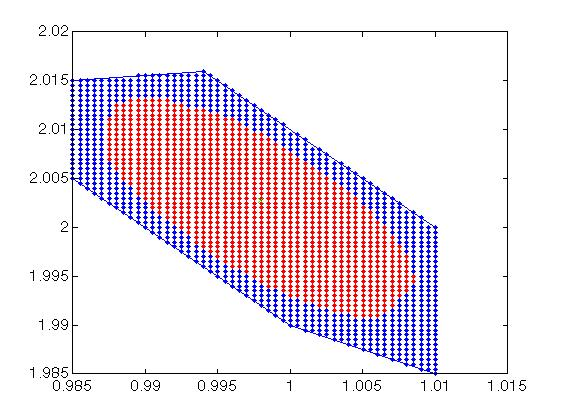
\includegraphics[width=.5\columnwidth]{Figures/confidenceRegionLR.jpg}}
 \caption{The 0.85 confidence region for a two parameter linear regression problem.}
 \label{fig:ConfidenceRegionLR}
\end{figure}

\subsubsection{testLTIConfidence.m}

This script is written to demonstrate that the SPS method indeed generates confidence regions with the required confidence level. A high number of membership queries are carried out for the nominal model on different confidence levels using different random noise values and SPS setups in each query. The membership answers are recorded and saved to the disk. The second part of the script visualizes the probability with which the nominal model was accepted to be in the confidence region or not.

After 15000 queries in each confidence level, the results are given in FIgure~\ref{fig:ConfidenceLR}.

\begin{figure}[htb]
 \centerline{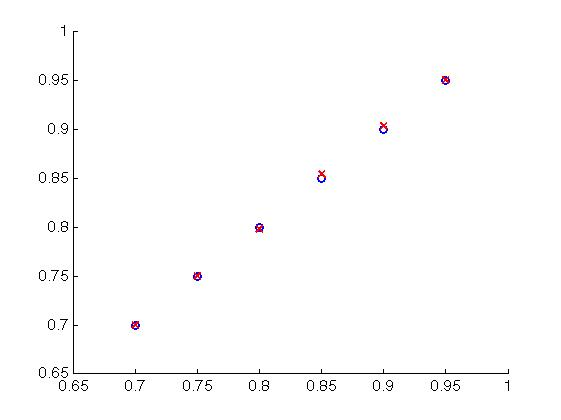
\includegraphics[width=.5\columnwidth]{Figures/confidenceLR.jpg}}
 \caption{The relative frequency of accepting the nominal model at given confidence levels (red) and the prescribed values for this (blue).}
 \label{fig:ConfidenceLR}
\end{figure}

\subsection{LTI systems}

\subsubsection{testLTIMembership.m}

Prediction error estimates always belong to the SPS confidence set as in their case $Z_0 = 0$. This script illustrates this by calculating the PEM estimate and checking its membership. The PEM estimate is calculated using the pem method in the Matlab System Identification Toolbox.

\subsubsection{showConfidenceRegion.m}

The structure of the confidence sets corresponding to a given SPS setup and data can be complex. This examples defines a fine grained grid around the PEM estimate of a selected two parameter model and evaluates the membership on every grid point. The sample code demonstrates how to generate and plot confidence regions in two dimensions, the result is given on Figure~\ref{fig:ConfidenceRegion}.

\begin{figure}[htb]
 \centerline{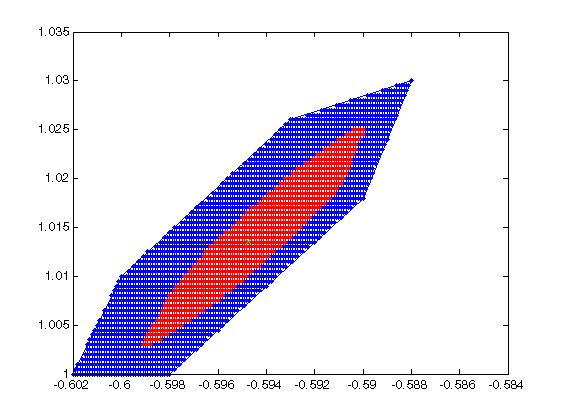
\includegraphics[width=.5\columnwidth]{Figures/confidenceRegion.jpg}}
 \caption{The 0.85 confidence region for a first order nominal system and output error noise model.}
 \label{fig:ConfidenceRegion}
\end{figure}

\subsubsection{testLTIConfidence.m}

This script is written to demonstrate that the SPS method indeed generates confidence regions with the required confidence level. A high number of membership queries are carried out for the nominal model on different confidence levels using different random noise values and SPS setups in each query. The membership answers are recorded and saved to the disk. The second part of the script visualizes the probability with which the nominal model was accepted to be in the confidence region or not.

After 15000 queries in each confidence level, the results are given in FIgure~\ref{fig:Confidence}.

\begin{figure}[htb]
 \centerline{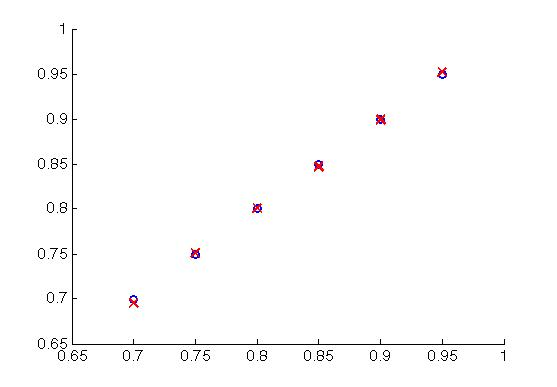
\includegraphics[width=.5\columnwidth]{Figures/confidence.jpg}}
 \caption{The relative frequency of accepting the nominal model at given confidence levels (red) and the prescribed values for this (blue).}
 \label{fig:Confidence}
\end{figure}

\pagebreak

\section{Deployment}
\label{sec:Deploy}

The code is available on GitHub using the following links: 
\begin{itemize}
\item GitHub repo history: \url{https://github.com/kolixx/SPSToolbox}
\item link for cloning the repo: \url{git://github.com/kolixx/SPSToolbox.git}
\end{itemize}

The different releases are contained in the root of the repo as archives containing the date of the release in the file name.

Add the folder SPSToolbox to the Matlab path collection using the menu "File/Set Path...". Mind that Matlab should be running with administrative privileges during this operation.

\bibliographystyle{ieeetr}
\bibliography{kolumban}

\end{document}




































